\Chapter{Ütközésvizsgálat}
\label{Chap:utkozesvizsgalat}

% TODO: Ütközéssel, metszéspontokkal kapcsolatos számítások

%- A try bullet-es példa részletes kifejtése, matematikai része

%Egyszerűbb változatoktól a bonyolultabbak fel

%- Először az intuitív, egyszerűbb megoldások, még ha kevésbé hatékony is.
%- Felsorolni több megoldást is.
%- Optimalizálási módszerek részletezése
%- Összehasonlítani őket pontosság és számításigény szempontjából.

Ebben a fejezetben az ütközésvizsgálattal kapcsolatos számításokról, optimalizációkról lesz szó. Ütközésvizsgálatra több szempontból is szükség van. Egyrészt, vizsgálni kell, hogy a játékos a játszható területen belül van-e, azaz nem mehet át falakon, tereptárgyakon, nem mehet fel túl meredek emelkedőn. Másrészt, vizsgálni kell, hogy a játékos által leadott lövedék eltalálja-e a domborzatot, tereptárgyakat, jelezni kell a lövedék becsapódását. Harmadrészt regisztrálni kell az ellenfeleket eltaláló leadott lövéseket. A második és harmadik pont nagyon hasonló, de még is szétszedtem, mert az ellenfeleknél nem a látható geometriát találjuk el, hanem annak egy leegyszerűsített modelljét, a számítások felgyorsítása érdekében. Szükség van további optimalizációkra is, mert ha ezek nem lennének, irreálisan nagy erőforrás igénye lenne a játékoknak.

\section{A karakterek ütközésvizsgálata mozgás szempontjából}

Ez a játék szempontjából az egyik legfontosabb elem. Az hogy kirajzoltatunk valamit a képernyőre, még nem jelenti azt, hogy azon nem lehet áthaladni. A kirajzolás csak a vizualitást adja, a domborzat, a tereptárgyak, a karakterek kinézetét. A játékfejlesztő feladata az, hogy megírja külön az ezekhez szükséges ütközésvizsgálatot. Mivel ez két különálló dolog, egyes helyzetekben adódhatnak olyan problémák, hogy ezek nincsenek szinkronban, tehát látunk valamit amin át lehet menni, vagy nem látunk valamit és mégis megakadunk benne.

Ebben a játékban a karakterek ütközésvizsgálata gradiens számítással van megoldva. Ez azt jelenti, hogy ha két, egymás mellett lévő pont magasságértéke között túl nagy a különbség pozitív irányba, az falat, vagy túl meredek emelkedőt jelent. Ha mérsékelt, vagy nagyon minimális a különbség, akkor arról vagy lecsúszik, vagy csak egyszerűen át lehet ott haladni. Mindezt a beolvasott magasságmezőből számolja, ezzel dinamikussá téve az ütközésvizsgálatot. Ha ez nem lenne így, akkor elveszne a játék azon tulajdonsága, hogy dinamikusan lehet cserélgetni a pályákat minden további nélkül. Az egyes számú algoritmusban a delta a különbséget, a h a magasságot, és a curr a jelenlegi értéket takarja. A lépték azt adja meg, hogy a következő pont milyen távolságra legyen, mennyire legyen pontos a számítás.

\begin{algorithm}[H]
 \KwData{delta; h; hx; hy; curr\_x; curr\_y; delta\_x; delta\_y\;}
 \KwResult{A meredekség számítása x és y irányban}
 	delta := térkép\_szélesség / (lépték * térkép\_szélesség);\\
 	h = altuális\_talajmagasság(curr\_x, curr\_y);\\
	hx := altuális\_talajmagasság(curr\_x + delta, curr\_y);\\
	hy := altuális\_talajmagasság(curr\_x, curr\_y + delta);\\
	delta\_x := (hx - h) / delta;\\
	delta\_y := (hy - h) / delta\; 
 \caption{Gradiens számolása}
\end{algorithm} 


Ezen felül a gravitáció ami nagyon lényeges, mert a pályának vannak olyan magaslati pontjai, amelyekre fel lehet jutni. Ha egy ilyenre felmegyünk, és nincs semmilyen erő, ami a karaktert a föld felé húzná, akkor felfelé ugyan lekövetné a talajmagasságot, de le már nem esne alacsonyabb pontra onnan.

Ez esetben egy lefelé ható erő folyamatosan hat a játékosra és ellenfelekre, aminek a küszöbértéke mindig az aktuális talajmagasság. Ugrás esetén a gravitációnál nagyobb, ellenirányú erőt fejt ki a karakter, amely folyamatosan csökken, ez eredményezi azt, hogy elemelkedik a földtől, egy ponton megáll, majd vissza is esik a talajra. Ez látható \aref{fig:gravity}-es ábrán. A gravitációs erő Fg-vel, a kifejtett erő Fk-val van jelölve.

\begin{figure}[h]
\centering
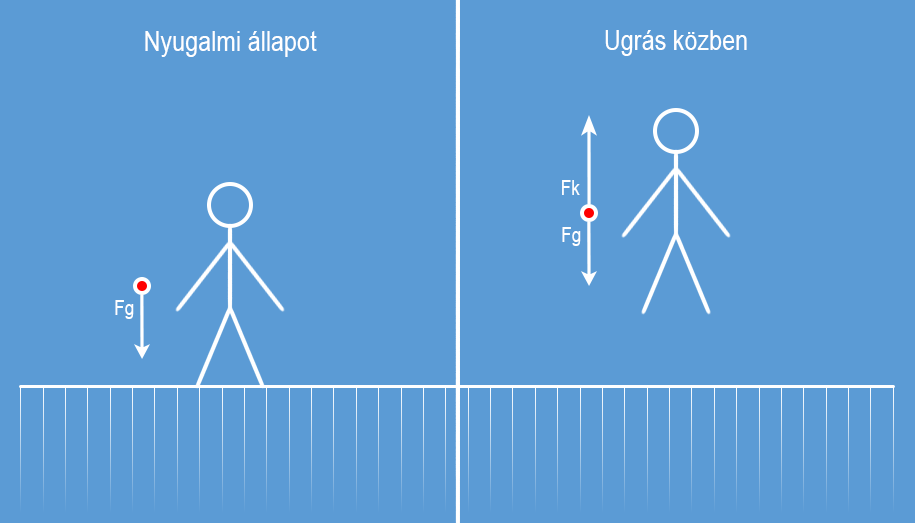
\includegraphics[scale=0.6]{kepek/gravity.png}
\caption{A karakterre ható erők}
\label{fig:gravity}
\end{figure}

\begin{algorithm}[H]
 \KwData{gravitációs erő; küszöbérték\;}
 \KwResult{A karakter föld felé húzása az aktuális talajmagasságig}
 küszöbérték := aktuális talajmagasság\;
  \eIf{karakter függőleges pozíciója > küszöbérték}{
   függőleges gyorsaság := függőleges gyorsaság + gravitációs erő\;
   karakter függőleges pozíciója := karakter függőleges pozíciója \\ + függőleges gyorsaság\;
   }{
   karakter függőleges pozíciója := küszöbérték\;
  }
 \caption{Gravitáció megvalósítása}
\end{algorithm} 
 
\section{A domborzat és tereptárgyak üközésvizsgálata a lövés szempontjából}

Az ilyen fajta ütközésvizsgálat számítás nem létszükséglet a játszhatóság szempontjából, de tény, hogy jóval realisztikusabbá teszi a játékot, és sok optimalizációt igényel. Ez teszi lehetővé, hogy ha lövünk egyet, és beletalál bármilyen elembe, ami a pálya része, megjeleníthessük rajta a találatot. Ennek minősége lehet többféle, csak egy textúra, vagy egyéb még realisztikusabb megoldások. Mivel a pálya háromszögekből áll, és az irány amerre nézünk egy egyenes, így itt egyenes és háromszög metszéspontját kell számolnunk térben. A pálya háromszöghálóját, geometriáját \aref{fig:wireframe} ábrán mutatom be.

\begin{figure}[h]
\centering
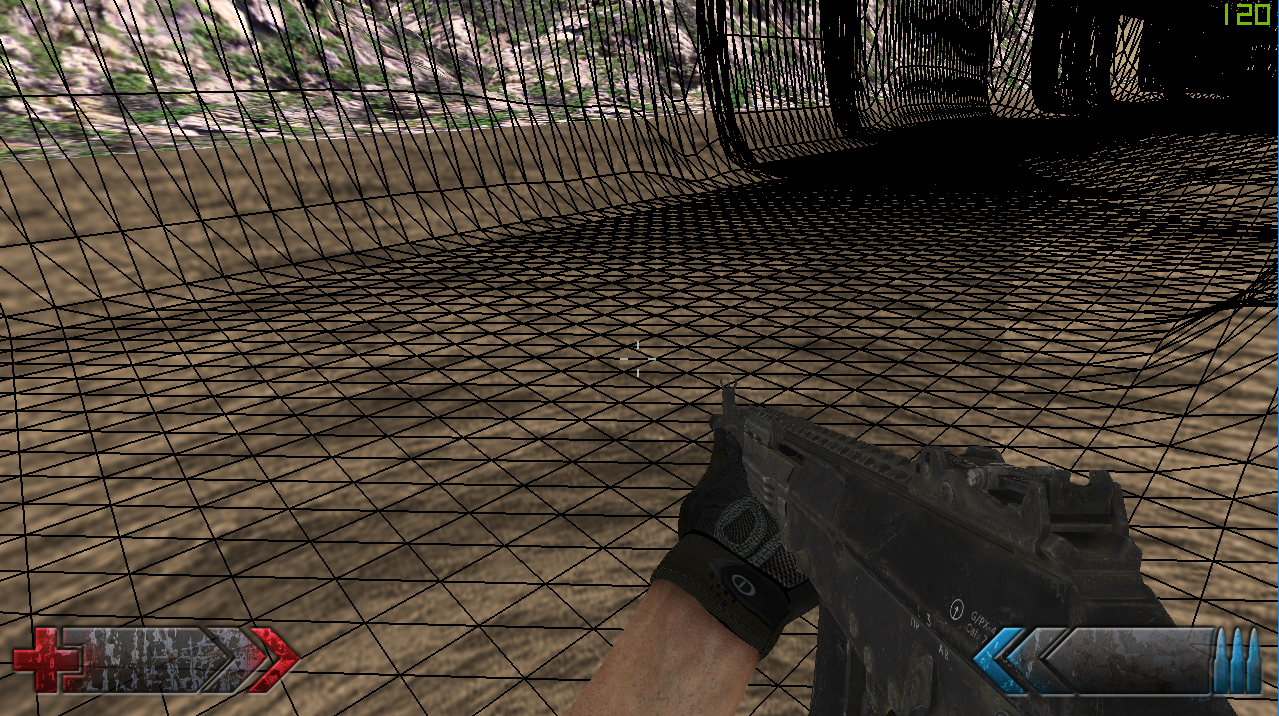
\includegraphics[scale=0.4]{kepek/map_wireframe.png}
\caption{A térkép geometriájának határvonalai}
\label{fig:wireframe}
\end{figure}

Első lépésként, meg kell határozni azt az egyenest, amely azt írja le, amerre néz az adott karakter. Ez az egyenes két ponttal van leírva. Az egyik az adott karakter pozíciójával egyezik meg. A másik, távoli pontot jelen esetben egy, az OpenGL-ben definiált függvényből, a GluLookAt-ből határozzuk meg, aminek 9 paramétere van. Az első három a karakter jelenlegi pozíciója, a második három azt a pontot írja le merre nézünk (referencia pont), az utolsó három pedig azt határozza meg, hogy melyik tengelyen, és merre néz a felfelé vektor. A 9 paraméter közül a középső háromból lehet a túlsó pontot  meghatározni. Mindegyikből ki kell vonni az adott tengelynek megfelelő jelenlegi pozíciót, majd megszorozni egy nagy értékkel, azért, mert ez nélkül túl közeli pontot kapnánk, ezáltal egy rövid egyenest.

Második lépés, ennek az egyenesnek kiszámolni a háromszögekkel való metszéspontját. A háromszögek a három csúcspontjukkal vannak leírva. Kell lennie egy függvénynek, amelynek a háromszög három csúcspontját, és az egyenes két végpontját átadva, visszaadja a metszéspont x,y,z koordinátáját. Ez működés közben \aref{fig:triangle} ábrán látható.

\begin{figure}[h]
\centering
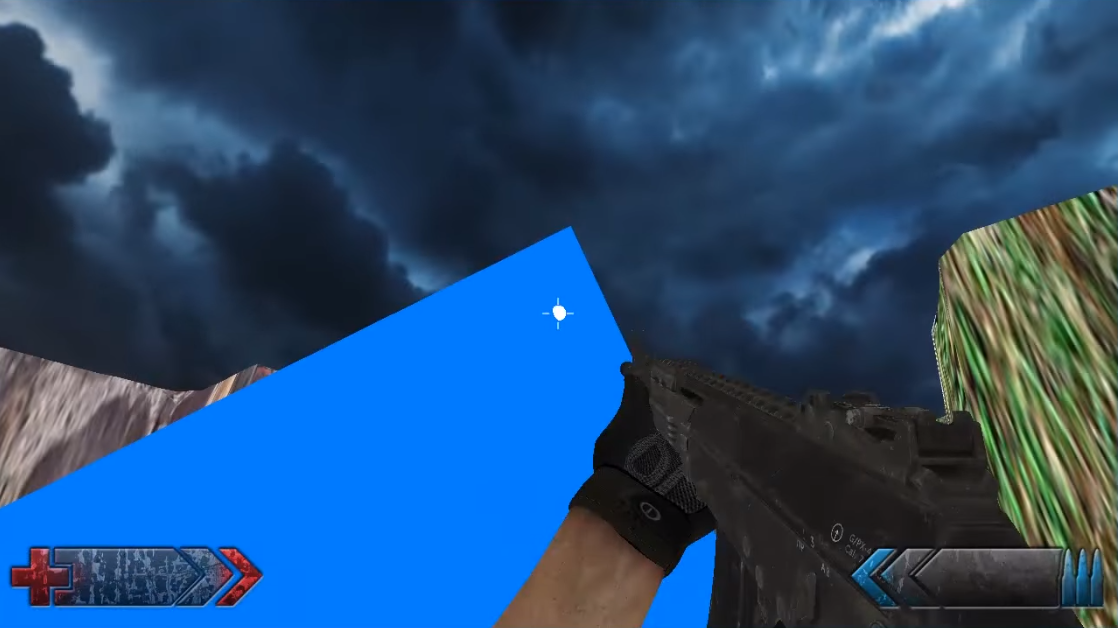
\includegraphics[scale=0.46]{kepek/one_triangle.png}
\caption{Egyenes és háromszög metszéspontja vizualizációval}
\label{fig:triangle}
\end{figure}

Ez a függvény először megvizsgálja, hogy azt a síkot, amelyen a háromszög van, metszi-e az egyenes, ha nem, nem is számol tovább. Ha metszi a síkot, akkor megnézi, pontosan hol metszi azt, megkapva az x,y,z koordinátákat. Ez után már csak azt kell vizsgálni, hogy a metszéspont benne van-e a három csúcspontjával leírt háromszögben. Ha igen, akkor visszaadja a pontos metszéspontot.

\section{A játékos, és az ellenfelek hitboxa}

% TODO: Hitbox kép linkét bemásolni a jegyzékbe
% http://www.toptiertactics.com/wp-content/uploads/2011/05/Hitbox.jpg 

Ennek alapelve ugyanaz, mint a domborzat és tereptárgyak üközésvizsgálatánál, annyi különbséggel, hogy itt azt kell vizsgálni, hogy az ellenfelek körül lévő, a játékosok számára láthatatlan hengerrel van-e metszéspontja az adott egyenesnek. Ezt a hengert nevezzük jelen esetben hitbox-nak, de egyéb játékokban lehet sokkal részletesebb, attól függően, mennyire szeretnénk pontosan regisztrálni az egyes találatokat.

\begin{figure}[h]
\centering
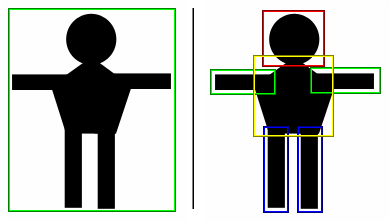
\includegraphics[scale=0.4]{kepek/hitbox.png}
\caption{Különböző részletességű hitbox-ok}
\label{fig:hitbox}
\end{figure}

Ebben az esetben azért nem a pontos, látható geometriára számoljuk a találatokat, mert annak nagyon nagy erőforrásigénye lenne, ellenben az lenne a legpontosabb, tehát amit látunk, az jelenti a találatot. A találatszámításra használt leegyszerűsített geometria előnye, hogy sokkal kevesebb hátérszámításra van szükség. Viszont mivel nem azt találjuk el, amit látunk, előfordulhatnak kellemetlen, vagy érdekes szituációk. Előfordulhat, hogy úgy találjuk el az ellenfelet, hogy ott valójában nem látunk semmit, vagy ennek ellenkezője, hogy elvileg eltaláljuk, de az a rész nem tartozik a hitbox-hoz.

Online lövöldözős játéknál a külön leegyszerűsített hitbox-os megoldással lehetnek még problémák. Ilyen például az, hogy a nem megfelelő internetkapcsolat okozta nagy válaszidő, vagy csomagvesztés miatt a hitbox elcsúszik a látható geometriától. Így akár hiába van leegyszerűsített, de még egész részletes geometria ráhúzva az adott karakterre, mégsem találjuk el az ellenfelet, mert az nem illeszkedik pontosan.

\section{Optimalizálási módszerek}

Mivel az ütközéskezelés során nagyon sok adattal kell számolni, szükség van optimalizációkra. Korábban ezt részben már említettem, hogy több százezer háromszög, vagy nagy terület esetén nagyon erőforrás igényesek a számítások, és teljesen fölöslegesen is számolja ki a processzor a teljes területre a ütközést, mikor a pálya túlsó felének közelében sem vagyunk. Erre létezik több optimalizálási mód, ilyen például a játéktér szabályos felosztása, a négyes fa vagy oktális fa.

\subsection{A játéktér szabályos felosztása}

Ez egy olyan módszer, amivel minden egyéb tényezőt figyelmen kívül hagyva felosztjuk a teret egy felosztási részletességet megadva. Meg kell adnunk, hogy melyik objektum, vagy a pályának melyik része melyik térrészben található, ez látható \aref{fig:grid} ábrán. A karakterek ütközésvizsgálatánál elég, ha mindig csak arra a térrészre vesszük figyelembe az ütközést amelyiken épp tartózkodik. Lövedék becsapódásának x,y,z koordinátáját is kevesebb számítással kaphatjuk meg így, mert csak azokat a térrészeket kell figyelembe venni, amelyek a játékos karakterének irányvektorával metszésben vannak. Előnye, hogy ezt a legegyszerűbb megadni, és ehhez képest elég nagy gyorsulást tapasztalhatunk. Hátránya viszont, hogy mindenhol egyformán osztjuk fel a teret, és lehetnek olyan részek, ahol indokolatlanul sűrű a felosztás. Ilyen például egy nagy mező, minden tárgy nélkül. Ennek kiküszöbölésére találták ki a négyes, és az oktális fát.

\begin{figure}[h]
\centering
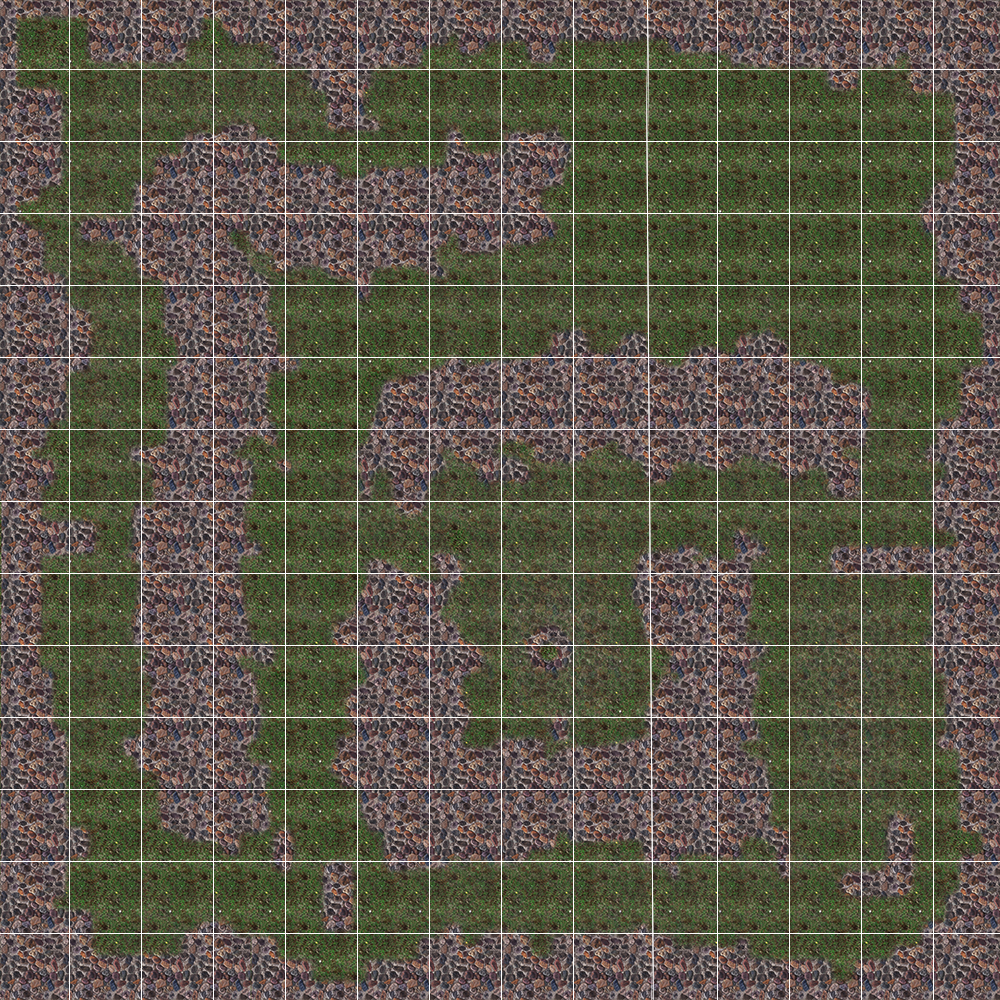
\includegraphics[scale=0.2]{kepek/grid.png}
\caption{A pálya felosztása egyenlő részekre}
\label{fig:grid}
\end{figure}

\subsection{Négyes fa és az oktális fa}

A négyes és az oktális fa ugyanolyan módszert takar, csak a négyes fát síkbeli, az oktális fát pedig térbeli felosztásra használják. Olyan, kivételes esetekben használható jól a négyes fa térben, ha a játéktér nem nagy magassággal rendelkezik. Használatánál az első feladatunk a fa gyökerének meghatározása, ami a teljes játékteret magában foglalja. Négyes fa esetén a síkot mindig 4 részre osztjuk mindaddig, még a fa mélysége el nem éri a maximális, előre definiált értéket, vagy az adott cellában az objektumok száma nem több mint egy előre definiált érték. Ugyanez a módszer érvényesül az oktális fánál, annyi különbséggel, hogy ott 8 felé osztjuk a teret. A négyes fa \aref{fig:quadtree} ábrán látható, hogyan is működik.

\begin{figure}[h]
\centering
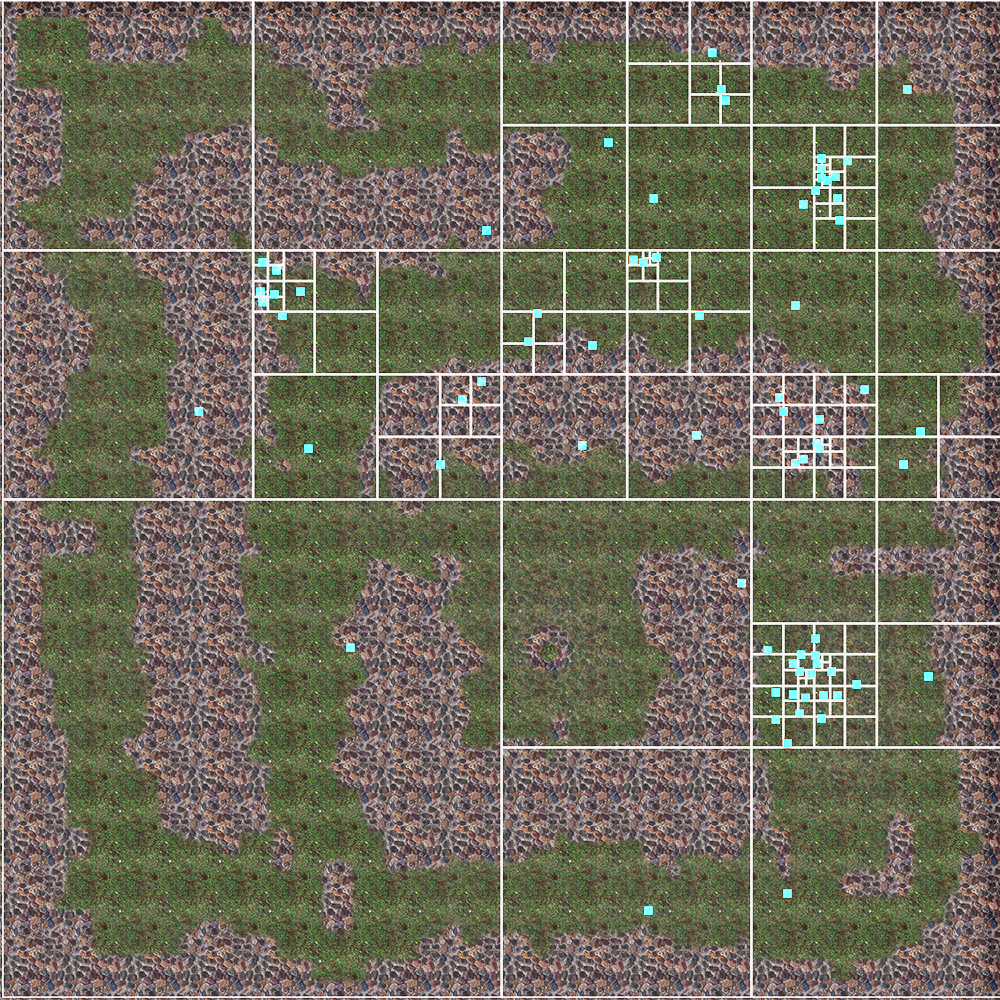
\includegraphics[scale=0.2]{kepek/quadtree.png}
\caption{A pálya felosztása a rajta lévő objektumok alapján}
\label{fig:quadtree}
\end{figure}

\subsection{Optimalizálási módszer kiválasztása}

A saját játékom készítése során a négyes fát alkalmaztam, hogy optimalizáljam az erőforrásigényt, a fölösleges számításokat mellőzve. Felvetődhet a kérdés, hogy miért négyes fát alkalmaztam, mikor a játék három dimenziós? Egyrészt azért, mivel ezt könnyebb megvalósítani. Másrészt, mint ahogy korábban is említettem, ha nincs a térnek nagy magassága, akkor tökéletesen elegendő lehet a négyes fa is, mivel az oktális fa ilyen esetben nem hoz annyival jobb eredményt, mint amennyivel több munka van vele.